\documentclass[tikz,border=2pt]{standalone}
\usepackage{amsmath,amssymb}
\usepackage{tikz}
\usetikzlibrary{arrows.meta}

\begin{document}
% A random variable is a function from the sample space to the real numbers: each outcome
% omega is sent to a number X(omega); here X = number of heads in two coin tosses.
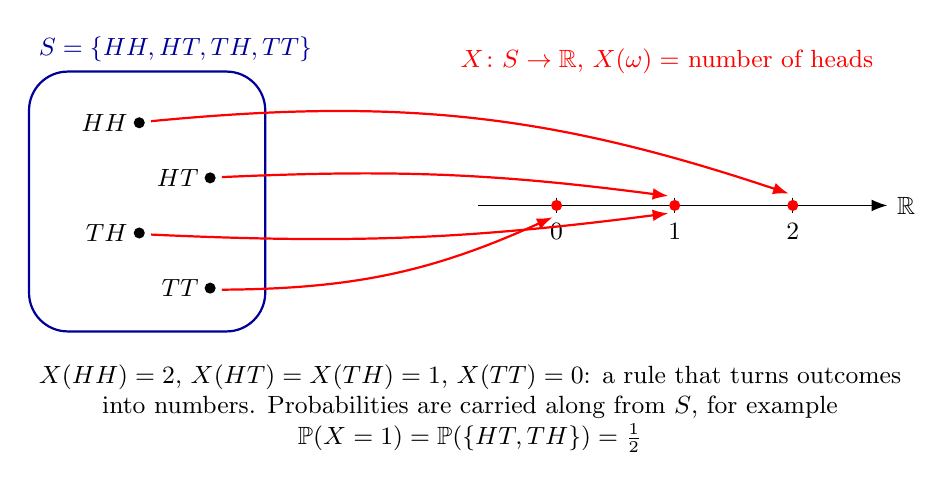
\begin{tikzpicture}[every node/.style={font=\small}, >={Latex[length=2mm]}]
	\draw[thick, blue!60!black, rounded corners=14pt] (-1.7,-1.6) rectangle (1.3,1.7);
	\node[blue!60!black, anchor=south west] at (-1.7,1.7) {$S=\{HH,HT,TH,TT\}$};
	\fill (-0.3,1.05) circle (2pt);
	\node[anchor=east, inner sep=4pt] at (-0.3,1.05) {$HH$};
	\fill (0.6,0.35) circle (2pt);
	\node[anchor=east, inner sep=4pt] at (0.6,0.35) {$HT$};
	\fill (-0.3,-0.35) circle (2pt);
	\node[anchor=east, inner sep=4pt] at (-0.3,-0.35) {$TH$};
	\fill (0.6,-1.05) circle (2pt);
	\node[anchor=east, inner sep=4pt] at (0.6,-1.05) {$TT$};
	\draw[->] (4,0) -- (9.2,0) node[right] {$\mathbb{R}$};
	\foreach \x/\l in {5/0, 6.5/1, 8/2} {\draw (\x,0.1) -- (\x,-0.1); \node[below=3pt] at (\x,0) {\l};}
	\draw[->, red, thick] (-0.15,1.07) to[bend left=12] (7.95,0.15);
	\draw[->, red, thick] (0.75,0.36) to[bend left=5] (6.42,0.12);
	\draw[->, red, thick] (-0.15,-0.37) to[bend right=5] (6.42,-0.1);
	\draw[->, red, thick] (0.75,-1.07) to[bend right=12] (4.95,-0.15);
	\foreach \x in {5,6.5,8} {\fill[red] (\x,0) circle (2pt);}
	\node[red, anchor=south] at (6.4,1.55) {$X\colon S\to\mathbb{R}$, $X(\omega)=$ number of heads};
	\node[anchor=north, align=flush center, text width=11cm] at (3.9,-1.9) {$X(HH)=2$, $X(HT)=X(TH)=1$, $X(TT)=0$: a rule that turns outcomes into numbers. Probabilities are carried along from $S$, for example $\mathbb{P}(X=1)=\mathbb{P}(\{HT,TH\})=\tfrac12$};
\end{tikzpicture}
\end{document}
